\begin{comment}
  What is the original framing of the problem? It almost doesn't make sense to frame it as a system-wide problem. Because a process is useless if it's totally isolated from the rest of the system. Make processes isolated and poke some holes in this isolation.

  This is something that has been on the radar since the origin of multi-processing
  systems.  We can argue that one of the reasons it's never been solved has been because
  the problem is too broadly defined.

  One set of tehcnologies that has helped in this sense has been hypervisor-based
  virtualization. But this is subject to some fundamental concerns. Containers

  It's a reframing but it's also narrowing the scope
  A "scoping definition"? A "scoping reframing"?
  Applying it specifically to containers and virtualization
\end{comment}


Researchers have been studying confinement for decades~\cite{lampson1973_confinement}, and
have been designing and applying confinement primitives since the early days of
time-sharing computers and multi-tenant systems~\cite{shu2016_security_isolation_study}.
While many developments have been made in the mean time, the current confinement landscape
(particularly within the Linux ecosystem) suffers from fundamental flaws that culminate in
poor container security practices; this does not need to be so. This chapter presents
a critique of the current state of confinement on Linux, examines how confinement
primitives are applied to containers, and proposes a fundamental re-framing of the problem
to focus on complexity, adoptability, and suitability for container-specific applications.
In light of this re-framing, we consider design goals for \bpfbox{} and \bpfcontain{} and
present the threat model for confinement under these research systems.

\section{Rethinking the Virtualization Narrative}%
\label{s:cp-rethinking}

Hypervisor-backed virtualization is commonly considered more secure than
con\-tain\-er-based virtualization~\cite{sultan2019_container_security,
eder2016_hypervisor_container} (see \Cref{fig:container-hvm-security}). Intuitively, this
makes sense.  Containers run directly on the host operating system, whereas a virtual
machine runs on top of a hypervisor, separated by at least one layer of indirection from
the host system.  However, this intuition does not strictly stand up to scrutiny.
A virtual machine running on top of a hypervisor makes requests to the hypervisor's
\gls{api} (via hypercalls), in much the same way as a container running on a host
operating system makes requests to the kernel's \gls{api} (via system calls).
\Cref{fig:syscall-hypercall} illustrates this parity. In both cases, a vulnerable
interface into a more privileged component of the system is directly exposed to the
attacker.

\begin{figure}[htbp]
  \centering
  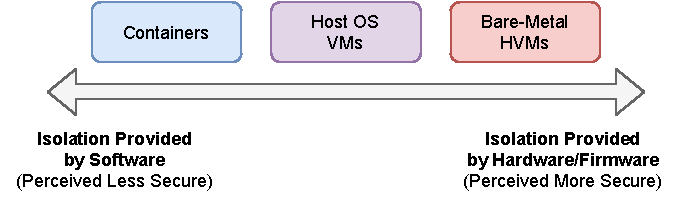
\includegraphics[width=0.8\linewidth]{figs/confinement-problem/security.pdf}
  \caption[Comparing the isolation and perceived security of containers and \glsentryshortpl{vm}]{
    Comparing the isolation and perceived security of containers and
    \glsentryshortpl{vm}. A boundary defined in hardware is often considered more rigid,
    whereas a software defined boundary is generally considered more malleable, and thus
    weaker. However, this need not be the case. The goal of this thesis is to reposition
    containers to be as secure, if not more secure, than hypervisor-based virtualization.
  }%
  \label{fig:container-hvm-security}
\end{figure}

\begin{figure}[htbp]
  \centering
  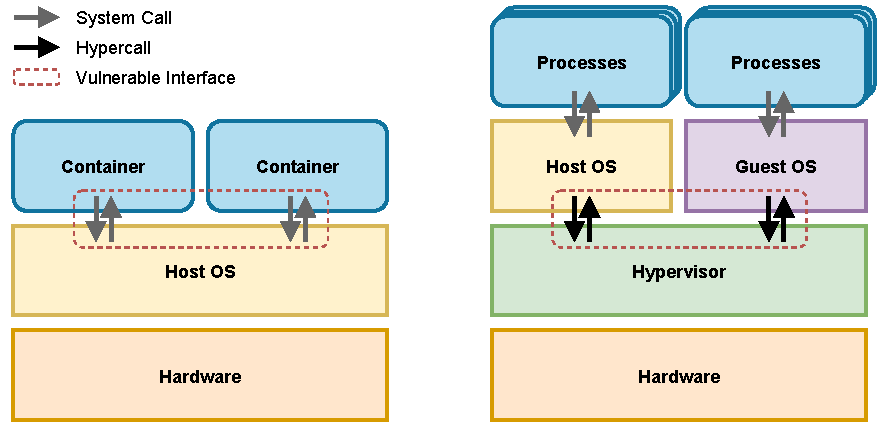
\includegraphics[width=0.8\linewidth]{figs/confinement-problem/syscall-hypercall.pdf}
  \caption[System calls and hypercalls as vulnerable interfaces]{
    System calls and hypercalls as vulnerable interfaces. Containers (which are really
    just process groups running on the host \gls{os}) make system calls to the
    more-privileged host \gls{os} kernel. Similarly, a guest operating system makes
    hypercalls to the more-privileged hypervisor. Both of these interfaces are ripe
    targets for a myriad of attacks, including privilege escalation and tampering with
    sensitive resources. This parity becomes particularly evident when we assume that an
    attacker has or is able to obtain control over the guest \gls{os}.
  }%
  \label{fig:syscall-hypercall}
\end{figure}

% The isolation guarantees provided by a virtual machine come almost entirely from a sense
% of obfuscation over a semantic gap, created as the hypervisor virtualizes system
% resources. There is no notion of centralized policy in a virtual machine; rather, security
% is an emergent phenomenon, a form of \enquote{policy through mechanism}. With the right
% tools, we can and have poked holes everywhere in this
% policy~\cite{dubrelle2015_hypervisor, thongthua2016_analysis, shahzad2017_systematic}.

In the case of virtual machines, security is an emergent phenomenon. The implicit
isolation provided by a virtual machine is purely a function of the semantic gap between
guest operating system, virtualized hardware, and physical hardware. Here, security is
intrinsically tied to functionality. Administrators poke holes in this isolation all the
time, through shared filesystems, virtual network interfaces, and the like. From there, it
is up to the administrator to use conventional \gls{os} security mechanisms
(c.f.~\Cref{s:process-security-model,s:security-extensions} in \Cref{c:background}) such
as filesystem access controls and network firewalls to lock down the exposed interface.
A clear pattern emerges: first provision the resource, then secure it, just as in an
ordinary operating system (after all, a guest operating system \textit{is} just an
operating system). The end result of this process is a combination of implicit isolation
and additional \gls{os}-level security mechanisms: a form of \textit{policy through
mechanism}.

The central argument of this thesis is that there is no fundamental reason why containers
cannot be as\,---\,if not more\,---\,secure than virtual machines.  While it is true that
a containerized process is nothing more than a host process running under one or more
\gls{os}-level virtualization primitives, an operating system that provides and enforces
the right set of confinement primitives should be able to lock a container down in much
the same way that a hypervisor implicitly enforces isolation.  Unlike hypervisor-based
isolation, such a policy enforced by the operating system has the potential to be more
minimal, centralized, and accessible to end-users. Further, we can attain a high level of
flexibility through a software-based enforcement mechanism, unencumbered by the
restrictions of a hardware-level interface.

The key to developing such an enforcement mechanism lies in defining a clear protection
boundary within the kernel and enforcing access across this boundary. Rather than
\textit{policy through mechanism}, this would be \textit{policy through exception}. Under
this model, the operating system enforces a clear protection boundary around the
container, and security policy then defines exceptions in this boundary, exposing
a minimal interface to the outside world.  Such an interface has the potential to be
\textit{far more minimal}  than that of a virtual machine, by taking advantage of the
fine-grained semantics exposed by the operating system.

However, the above depiction of container security does not match the current reality.
Existing container runtimes simply reuse confinement primitives exposed by the operating
system, combining multiple \gls{os}-level security mechanisms to secure specific system
resources.  This approach is neither simple nor unified, and results in increasingly
complex and verbose policies, inundated with the technical baggage associated with locking
down an entire operating system. Yet it is hard to fault the designers of container
runtimes for this design choice; a container runtime's job is to run containers, not to
implement new security mechanisms. Intuitively, it makes sense to reach for primitives
that already exist, regardless of the fact that these primitives may have been designed
for system-wide use cases, beyond individual processes or even process groups. Likewise,
the goal of this thesis is not to design a new container runtime\,---\,rather, it is to
implement the missing confinement mechanism that will enable our vision for container
security to become a reality.

Before we can address concrete goals for such a confinement mechanism
(c.f.~\Cref{s:cp-design,s:cp-threat-model}), it is important to understand the fundamental
issues underlying the current state-of-the-art in Linux confinement and container
security. To that end, \Cref{s:cp-issues} outlines three main issues with current Linux
confinement primitives and \Cref{s:cp-containers} examines and critiques how container
runtimes apply these primitives in practice.

% The primary difference between the two is where and how the security boundary is
% defined.  In the case of containers, the boundary is defined in software, by \gls{os}
% security mechanisms; in the case of a hypervisor, the boundary may be defined in software,
% hardware, or firmware.

% \todo{You can't craft fine-grained policies with a virtual machine. You get a box. Network
% firewalls, shared filesystem with access controls. (The cognitive overhead to lock down
% a virtual machine after exposing specific interfaces is very high.) With a virtual machine,
% policy is intrinsically tied to functionality. It's all about configuring the interfaces
% and then locking it down (either from the inside or outside). Provision the resource and
% secure it, because that's how you do it with a conventional operating system. Here, the
% provisioning is already taken care of by the operating system, so all we're doing is
% specifying the access.}

% \todo{Verify the following: VM escapes are partially about exploiting bugs, but it's also
% that the attacker has access to a lot of functionality that allows them the opportunity to
% exploit these bugs. It's not least-privilege. You're giving them an entire VM. They have
% control over the entire OS and the entire hardware interface becomes an attack surface. In
% principle, with a container, you can make this exposed interface very small. People think
% of the hardware interface as being more secure, even though in principle it is larger,
% since it is rigid. But we have a hard boundary in the Linux kernel too: the \gls{lsm}
% layer. People think of hardware as being more secure, and somehow they think this notion
% carries forward to hardware semantics implemented in software.}

% \todo{Talk about why containers suck in brief and lead into 3.2}
% \todo{We have a repeated mistake here: Taking the interface that's there as the one we use
% to define our security properties. When we build containers, we made the mistake again of
% thinking that the interfaces are rigid, and that we need to make use of the abstractions
% that already exist. For the people who are designing container runtimes, their goal is to
% design container runtimes, not reinvent security mechanisms. Our goal is not to design
% a new container runtime, it's to improve the security of existing runtimes.}


% \begin{inprogress}
%   \begin{itemize}
%     \item Just like the word container makes people think about security
%     \item Type I and Type II hypervisor, the way it's depicted, makes people think something else is happening
%     \item The representation and terminology
%     \item This makes sense to talk about it if we connect it to containers
%     \item Why can't containers give as good or better security than hypervisors
%     \item Can we just get our enforcement clear
%     \item Virtual machines seem like they define a clear boundary, but it isn't actually
%           so clear in practice because all these things are being shared across boundaries
%     \item People think of virtual machines as being inherently more secure, the security
%           benefit is more of an obfuscation thing related to the semantic gap but with the right
%           tools you can still cross it freely
%     \item VMs have all these little holes everywhere and the policy is not centralized\,---\,we
%           have policy through mechanism
%     \item There's no reason why containers can't be as (if not more) secure than virtual machines
%     \item Because we can make this boundary very clear
%     \item \bpfcontain{} can be seen as a step towards this
%   \end{itemize}
% \end{inprogress}



\section{Fundamental Issues with Linux Confinement}%
\label{s:cp-issues}

Here we identify three fundamental issues with the current state of Linux confinement and
contextualize them with examples from existing container and confinement frameworks. This
section serves to provide additional context for the container-specific issues discussed
in \Cref{s:cp-containers}, and the design goals for \bpfbox{} and \bpfcontain{}, discussed
in \Cref{s:cp-design}.

\begin{enumerate}[font=\bfseries]
  \item \label{i:problem-complexity} \textbf{Complexity, Interdependence, and Inflexibility.}
    Existing confinement primitives are overly complex and designed for use cases beyond
    simple process confinement. To achieve simple confinement, frameworks must abuse and
    recombine a number of existing primitives, each designed for a different use case.
    Namespaces~\cite{biederman2006_namespaces, linux_namespaces} were designed to
    virtualize resources; they do not provide confinement by themselves. To truly confine
    a process using namespaces, we need a way to account for namespace escapes.
    Cgroups~\cite{cgroups}, similarly, were designed to virtualize the availability of
    quantifiable resources, not to directly confine. Unix
    \gls{dac}~\cite{jaeger2008_os_security, van_oorschot2020_tools_jewels} is far too
    coarse-grained and easy to bypass to be directly useful for confinement. POSIX
    capabilities~\cite{posix_capabilities} can be used to reduce overprivilege by
    partitioning root privileges, but these do not implement confinement by themselves.

    Seccomp-bpf~\cite{seccomp, edge2015_seccomp} works well to reduce the attack surface
    exposed by system calls, but writing classic \gls{bpf} filters is a complex and
    error-prone process. Fine-grained filtering quickly becomes untenable, particularly
    when considering race conditions when checking system call arguments and system call
    equivalence classes.  Linux \gls{mac} can be used to implement true confinement, but
    a typical \gls{lsm} like AppArmor~\cite{cowan2000_apparmor} or
    SELinux~\cite{smalley2001_selinux} is designed for use cases beyond simple sandboxing.
    These mechanisms are designed to implement and enforce system-wide \gls{mac} policy,
    not simple process-level confinement~\cite{belair2019_leveraging}. Further, major
    \glspl{lsm} are statically loaded and unstackable, meaning that end-users must
    generally choose one major solution with little room to adjust enforcement at runtime.

    To implement confinement, sandboxing and containerization frameworks generally mix and
    match the aforementioned solutions\,---\,some of which were designed for confinement,
    some of which were not, and none of which were designed for \textit{simple,
    process-level} confinement. LXC, Docker, Snap, and others all combine namespaces,
    cgroups, capabilities, seccomp-bpf, and AppArmor/SELinux policy to achieve
    confinement. In the case of Snap, high-level abstractions in policy definition can
    simplify the process of policy authorship to a certain extent, but simple policies
    are still compiled down into thousands of lines of policy soup, spanning multiple
    confinement mechanisms.

  \item \label{i:problem-unsuitability} \textbf{Unsuitability for Containers.}
    Existing Linux \gls{dac} and \gls{mac} is unsuitable for containers.
    \gls{lsm}-based \gls{mac} implementations like AppArmor and SELinux are
    designed to implement global, system-wide confinement policy; they are not designed
    for ad-hoc, process-level confinement~\cite{belair2019_leveraging}. Additionally,
    these \gls{lsm} implementations were not designed with containers in mind and thus
    do not consider container semantics in policy definition and enforcement. This lack
    of semantic awareness further complicates policy authorship for containers and
    forces the end-user to make compromises between security and functionality.

    Sultan \etal~\cite{sultan2019_container_security} suggest that the container
    security community should move towards a container-specific \gls{lsm}
    implementation. Security namespaces, proposed by Sun
    \etal~\cite{sun2018_security_namespace} can be seen as a partial step toward solving
    this problem.  Under security namespaces, each container can load and use its own
    \gls{lsm} of choice, but these \glspl{lsm} would still be subject to many of the
    same aforementioned restrictions. That is, existing \glspl{lsm} are not designed
    with container semantics in mind. A truly container-specific \gls{lsm} could incorporate
    container semantics into policy enforcement for cleaner and more effective policies.

    \gls{uid} remapping under a new user namespace does help with the \gls{dac} case by
    remapping root to a non-root \gls{uid}, but this is only really helpful for limiting
    the power of root. Other limitations of \gls{dac} still apply. For instance,
    a world-readable file could still be used for information disclosure or
    a world-writable file could still be the target of data corruption. For such reasons,
    \gls{dac} alone appears to be fundamentally insufficient for true isolation between
    host and container. Thus, to achieve proper process-level confinement for containers,
    we need an \gls{lsm}-based solution that is aware of container semantics.

  \item \label{i:problem-adoptability} \textbf{Difficulty Adopting New Solutions.}
    Motivated by the inherent difficulties associated with the existing confinement space,
    academics are often tempted to propose new confinement solutions. Many try to solve
    the problem by simply recombining and reusing existing primitives in new and
    innovative ways.  However, these types of solutions generally are not really a step
    forward with respect to addressing the issues in items 1 and 2, since these are
    emergent properties inherent to the underlying confinement primitives themselves.

    In order to truly solve these fundamental issues, we need kernel support for new
    primitives. Unfortunately, this begets yet another fundamental issue: adding new
    solutions directly to the kernel is difficult, particularly from an adoptability
    standpoint. New kernel code can introduce bugs and security vulnerabilities, and needs
    to be thoroughly tested before it can be considered production ready. Paradoxically,
    the potential to introduce new security vulnerabilities can make the use of such novel
    primitives \textit{less} secure. Similarly, kernel bugs can introduce availability
    concerns in production systems, even when such bugs are not security-critical. For
    these reasons, industry managers may be reluctant to adopt new, out-of-tree solutions
    based on loadable kernel modules, for example~\cite{gregg2019_bpf}.

    Another adoptability concern arises when we consider \textit{container-specific}
    confinement~\cite{sultan2019_container_security, sun2018_security_namespace} as an
    end-goal.  To date, the definition of precisely what a container is has been more or
    less in flux. The requirements and precise specifications of what constitutes
    a container tend to change as container frameworks evolve and new use cases crop up.
    If not everyone can agree on what a container even is, how can we expect to reach
    agreement on which underlying container security abstraction should be merged into the
    mainline kernel? To solve this problem, we need a way to add abstractions into the
    kernel in such a way that is neither binding nor limited by the lack of adoptability
    associated with traditional kernel-based solutions. These requirements motivate the
    use of \gls{ebpf} for designing a container-specific security solution, and thus
    motivate the design of \bpfbox{} and \bpfcontain{}.
\end{enumerate}



\section{How Containers Apply Confinement Primitives}%
\label{s:cp-containers}

This section examines and critiques the way Linux container technologies apply confinement
primitives to lock down container deployments. We focus primarily on Docker as a case
study, however these principles in general apply to the majority of container management
frameworks.

In general, Linux containers have three broad goals. However, these goals are neither
equally met nor equally prioritized by existing container management frameworks. In order
of decreasing prioritization, they are:
\begin{enumerate}[font=\bfseries]
  \item \textbf{Dependency Management / Reproducibility.}
    Containers should provide an easy and robust framework for creating reproducible
    development environments. Dependencies should be maximally self-contained such that
    a containerized environment \enquote{just works} to the maximum possible extent. We
    can see examples of this property in Docker, the predominant container framework at
    the time of writing. Docker Hub~\cite{docker_hub} allows container images to be pulled
    from the Internet, recombined, and used to create further images. The end result is
    a flexible framework for creating and distributing reproducible development
    environments.

  \item \textbf{Virtualization.}
    Containers should virtualize system resources, creating the illusion of running on
    a separate physical machine. Where possible, resources should be transparently reused
    between multiple containers (e.g.~sharing a single base copy of the same shared
    library between two container images).

    To achieve virtualization, containers generally rely on the namespaces and cgroups
    primitives provided by the Linux kernel.  Overlay filesystems~\cite{overlayfs}
    combined with the mount namespace allow containers to perform one-way sharing of
    filesystem resources. The \gls{pid} namespace allows each container to have its own
    \textit{init} process and virtual process tree.  The network namespace allows the
    container to virtualize its network devices while the \glsentryfull{uts} namespace
    virtualizes host and domain names. Control groups virtualize other resources such as
    the \gls{cpu}, main memory, and device drivers.

  \item \textbf{Confinement.}
    Containerized processes should be confined by default. That is, a containerized
    process should have access to the minimal set of privileges required for it to operate
    normally. Container runtimes leverage existing confinement primitives provided by the
    operating system, when available, to confine themselves. However, the extent to which
    this property is achieved varies greatly, both by the specific container runtime and
    by the characteristics of the deployment
    environment~\cite{sultan2019_container_security, lin2018_container_security,
    bui2015_docker_analysis}. In general, proper confinement is not a high priority of
    container runtimes, and this tends to result in sacrificing security for ease of
    deployment.
\end{enumerate}

The aforementioned goals are not only ordered by their decreasing prioritization in extant
container management frameworks; they are also ordered by increasing relevance to
container security. That is to say, existing frameworks generally prioritize goals
unrelated to security and leave security as an afterthought. Since containers are really
just process groups running directly on the host operating system, an unconfined container
therefore exposes the same attack surface as an ordinary host process. Thus, one might
expect container security to be of paramount importance. Unfortunately, this is not the
case. These difficulties in confinement motivate the need to revisit container security
and approach it from a confinement-first perspective. To understand how these confinement
issues impact containers, we briefly review how container management systems apply
confinement primitives in practice.

To achieve confinement in the first place, container frameworks cobble together existing
confinement technologies and apply them ways that are often simultaneously confusing and
difficult to audit. The result is a complex policy soup with little room for customization
or auditability. \Cref{i:problem-complexity} in \Cref{s:cp-issues} outlines some examples
of the inherent complexity that arises from mixing and matching confinement primitives in
this way. To deal with this complexity, some container runtimes elect to use a high-level
policy language that compiles down to thousands of lines of policy under the hood. Snap~\cite{snap}
is one such mechanism. Docker~\cite{docker_security, docker_default_apparmor, docker_apparmor} instead
elects to use an overly-permissive, generic policy template to avoid the potential issues
associated with fine-grained policy defaults.

% For instance, Snap~\cite{snap} uses a high-level policy language that
% targets system interfaces in a coarse-grained manner. Under the hood, this is compiled
% into hundreds or thousands of lines of seccomp-bpf and AppArmor policy.
% Docker~\cite{docker_security, docker_default_apparmor, docker_apparmor} uses a generic
% AppArmor, seccomp-bpf, and POSIX capability policy for every container, along with default
% namespace and control group configurations. Making meaningful changes to these policy
% configurations, beyond simply disabling them altogether, is difficult and
% error-prone~\cite{lin2018_container_security}.

Container security policies are often overly-generic and ill-suited to fine-grained
confinement. Part of the problem here is that containers in general are designed to
\enquote{just work}. Overly fine-grained security policies may get in the way of this,
particularly as end-user requirements vary and evolve across deployments.
Docker~\cite{docker_security}, for instance, provisions an overly-permissive default
AppArmor policy~\cite{docker_default_apparmor} designed to enforce basic protections
against interacting with sensitive kernel parameters without impacting the functionality
of the container.

Even worse, many container management systems operate under a fail-open approach when the
necessary security mechanisms are not supported. This results in low-security deployments,
often without even notifying the user that there may be such a configuration. Since the
end-user generally doesn't even participate in the policy authorship process, they may not
even be aware of the level of protection that is being applied, resulting in a dangerous
false sense of security. Docker's AppArmor policy~\cite{docker_apparmor,
docker_default_apparmor}, for instance, is not applied when the deployment environment
doesn't support AppArmor or AppArmor is disabled. Snap~\cite{snap} and others that rely on
the AppArmor or SELinux \glspl{lsm} for confinement suffer from similar failings.

Other aspects of confinement policy may be ignored entirely or even worse, overridden by
a more permissive policy, possibly without the user's knowledge.
Docker~\cite{docker_security} applies a dangerously permissive \texttt{iptables} policy
that can transparently expose a container to an external network, even overriding existing
deny rules. This overly-permissive network policy was the direct cause of a recent data
breach at NewsBlur~\cite{newsblur}, a news aggregation website, although NewsBlur
administrators claim that no user data was actually compromised~\cite{newsblur}.



\section{Design Goals}%
\label{s:cp-design}

% Unlike hypervisor-based isolation, a policy enforced by the operating system has the
% potential to be more minimal, centralized, and accessible to end-users. The key to
% developing such an enforcement mechanism lies in defining a clear protection boundary
% within the kernel and enforcing access across this boundary. \bpfbox{} lays the foundation
% for such an enforcement mechanism, and \bpfcontain{} explicitly applies it to containers.

To rectify the issues discussed in \Cref{s:cp-issues} and \Cref{s:cp-containers}, this
thesis introduces two novel confinement mechanisms, \bpfbox{} and \bpfcontain{},
implemented using \gls{ebpf}. \bpfbox{} (c.f.~\Cref{c:bpfbox}) is a sandboxing framework
that enables the definition of simple yet precise per-application policies that can be
dynamically loaded and enforced at runtime. Leveraging \gls{ebpf}'s system
introspection capabilities, \bpfbox{} policies can specify rules that span userspace and
kernelspace, targeting behaviours at the per-function-call level and enforcing policy
through \gls{lsm} hooks.

\bpfcontain{} (c.f.~\Cref{c:bpfcontain}) extends \bpfbox{} to model container semantics,
enabling it to clearly define a hard boundary around containerized processes.
\bpfcontain{} policies then define explicit exceptions to the default protection boundary,
offering fine-grained control over the interface that a container exposes to the outside
world.

The ultimate goal of \bpfbox{} and \bpfcontain{} is to expose centralized, flexible
policies that are simple enough for an end-user to perform ad-hoc confinement. In the case
of \bpfcontain{}, this goal is further extended to promote the adoption of
container-specific policies that isolate by default and can be extended to support
inter-container communication and resource sharing. To guide \bpfbox{} and \bpfcontain{}
toward this goal, we consider three primary design goals, derived from the fundamental
issues identified in \Cref{s:cp-issues}. They are enumerated as follows.

% In \bpfcontain{}, a clear and well-defined abstraction for containers
% allows the kernel to enforce implicit policy centred around container semantics. We rely
% on \gls{ebpf} to enable the definition of such an abstraction without necessarily tying
% the kernel down to one specific interpretation of what a container actually is. Using
% multiple \gls{ebpf} programs and maps, we can combine various other aspects of system
% behaviour with \gls{lsm}-based enforcement in a stateful manner. \bpfbox{} uses its
% ability to introspect system state to enable policy enforcement at the granularity of
% individual function calls.

% \todo{Rephrase this: Our goal is to have policies that are centralized, flexible, ...}
% In \bpfbox{}, policies are defined in a centralized, flexible policy file. Using
% \gls{ebpf}, \bpfbox{} can observe various aspects of system behaviour, such as user and
% kernelspace function calls, and incorporate them into its enforcement decisions. This
% helps define fine-grained policy while keeping the overall policy syntax clean and simple.
% \bpfcontain{} extends this model by defining an implicit protection boundary around
% a container, where the container is made up of a set of host processes and associated
% resources. Operations \textit{within} the container are implicitly allowed, whereas
% operations \textit{outside} the container or operations that can affect the system as
% a whole are implicitly denied. In this way, \bpfcontain{} policy allows the user to define
% \textit{exceptions to implicit rules} rather than the rules themselves.

% At this point, it should be clear that both \bpfbox{} and \bpfcontain{} leverage the power
% of \gls{ebpf} to make improvements on the existing status quo of Linux confinement. The
% next two sections, \Cref{s:cp-issues} and \Cref{s:cp-containers}, discuss the state of
% confinement on Linux and how existing container technologies apply confinement primitives.
% This discussion serves to contextualize the notions behind this section and motivates the
% need for \bpfbox{} and \bpfcontain{} as novel confinement primitives.

% \todo{Revisit this:}
% Using the above analysis of the confinement problem, we can derive a clear set of design
% goals for \bpfbox{} and \bpfcontain{}, such that they approach a solution to issues that
% plague the status quo. In particular, we derive the following three design principles.
% Note that these design principles are each the polar opposite of the three major problems
% identified in \Cref{s:cp-issues}.

\begin{enumerate}[font=\bfseries]
  \item \label{i:dg-simplicity} \textbf{Simple and Flexible Policies.}
    Policies should be simple and flexible, without sacrificing expressiveness. It should
    be possible to use our solution for ad-hoc confinement of individual
    applications and containers, without worrying about the underlying details of
    enforcement. At the same time, the policy language and enforcement engine should be
    flexible enough to support expressive and fine-grained policies that target specific
    system resources where required. That is, the barrier to entry for writing an
    effective security policy should be low, yet it should still be possible to write
    a sophisticated security policy where needed. Further, the policy enforcement engine
    underlying our confinement solution should be readily extensible, such that new
    kernel interfaces and policy rules can be easily supported as required.
    % \bpfbox{} and \bpfcontain{} should be simple, self-contained, and flexible.  The
    % policy language for each should be as simple as possible without sacrificing
    % expressiveness, and should not rely on any manual labelling of system resources as in
    % SELinux~\cite{smalley2001_selinux}. \bpfbox{} and \bpfcontain{} should be able to
    % fully confine a process without the relying on additional confinement primitives; that
    % is, the enforcement engines underlying \bpfbox{} and \bpfcontain{} should be fully
    % self-sufficient.

    % The policy language for \bpfbox{} and \bpfcontain{} should be as flexible as possible,
    % supporting multiple distinct use cases from basic sandboxing, to addressing specific
    % vulnerabilities in an application, to full-fledged container deployments. Using
    % \gls{ebpf}, \bpfbox{} and \bpfcontain{} can incorporate additional system state into
    % enforcement decision, beyond the state exposed by \gls{lsm} hooks.

    % The ultimate goal of \bpfbox{} and \bpfcontain{} is to make fine-grained confinement
    % accessible to the end-user, without the need to rely on complex configuration,
    % unnecessary setup, or the combination of multiple confinement primitives.

  \item \label{i:dg-suitability} \textbf{Suitable for Containers.}
    Our confinement solution should be suitable for containers. To support this goal, the
    policy language should encourage the authorship of light-weight, localized policies,
    tailored to specific use cases rather than a heavy-weight, system-wide \gls{mac}
    policy.  An ideal policy language for this purpose should be designed with container
    semantics in mind, enforcing a strong boundary around a container and related
    resources. To support inter-container communication and resource sharing, such
    a policy language should support the ability to selectively define exceptions to this
    boundary, as required.
    % \bpfbox{} and \bpfcontain{} should be suitable for process-level and container-level
    % enforcement respectively. The policy language design should encourage the authorship
    % of light-weight, localized policies, tailored to a specific use case, rather than
    % a heavy-weight, system-wide \gls{mac} policy. In the case of \bpfcontain{}, its policy
    % language and enforcement engine should also be designed with container semantics in
    % mind, enforcing a strong implicit boundary around a container and related resources.
    % To support inter-container communication and resource sharing, \bpfcontain{} should
    % provision the ability to define exceptions to this implicit boundary as required.

  \item \label{i:dg-adoptability} \textbf{High Adoptability.}
    % As a novel security mechanism, adoptability is of paramount importance. Without adoptability,
    % any security guarantees provided by such a mechanism would be effectively useless.
    Our confinement solution should be readily adoptable, even in production environments.
    All privileged code should be verifiably production-safe and should not negatively
    impact the rest of the system when loaded into the kernel. Performance overhead should
    at least be in line with alternatives like SELinux and AppArmor and our solution
    should work out of the box on a vanilla Linux kernel, without requiring any
    out-of-tree kernel patches or modules.
    % Both \bpfbox{} and \bpfcontain{} should be readily adoptable in production
    % environments, the cloud, and even personal desktop environments. In particular, the
    % requirements to run these mechanisms should be minimal, all privileged code should be
    % safe to use in production, system overhead should be in line with existing confinement
    % mechanisms, and both \bpfbox{} and \bpfcontain{} should work out of the box on an
    % unmodified, vanilla version of the Linux kernel.

    % To support these goals, \bpfbox{} and
    % \bpfcontain{} leverage the adoptability guarantees provided by \gls{ebpf} along with
    % a modular design that focuses on simplicity. For additional security, \bpfbox{} and
    % \bpfcontain{} support confinement without requiring setuid root binaries and all ring
    % 0 code passes through the \gls{ebpf} verifier before it is loaded into the system.
\end{enumerate}

The key insight behind this work is that novel \textit{kernel-level mechanisms} are
required to realize the aforementioned design goals. \gls{ebpf} provides precisely the
right framework for developing such mechanisms. Its safety, compatibility with vanilla
Linux kernels, and the ability to dynamically load and unload programs all contribute to
strong adoptability guarantees. The ability for distinct program types to use \gls{ebpf}
maps to communicate and share state enables the development of powerful confinement
solutions that can unify policy across disparate interfaces. Using \gls{ebpf}, we can
trace individual userspace and kernel function calls, along with the entire lifecycle of
a process or container. This property enables the creation of a fine-grained policy
enforcement mechanism that can easily be adapted and extended to support new semantics and
kernel interfaces as required.



\section{Why Two Implementations?}
\label{s:cp-why-two}

In light of the design goals outlined in \Cref{s:cp-design}, we now examine why this
thesis presents \textit{two} confinement implementations, rather than just one. The simple
explanation for this is that \bpfbox{} can be seen as a rough, first cut at solving the
confinement problem described in this chapter. Rather than a completely new system,
\bpfcontain{} should be seen as an \textit{iteration} on the original \bpfbox{} design.
In particular, \bpfbox{} satisfies each of the design goals enumerated in
\Cref{s:cp-design} to varying degrees; \bpfcontain{} improves upon this by further
simplifying the policy language, introducing container-level policy semantics, and
improving adoptability by leveraging \gls{bpf} \gls{core} (c.f.~\Cref{ss:bpf-userspace} in
\Cref{c:background}).

Thus, \bpfbox{} and \bpfcontain{} should not be seen as competing or even complementary
solutions to the confinement problem. Rather, the delta from \bpfbox{} to \bpfcontain{} is
representative of the intellectual journey from a first approximation to a far more
refined approach, more conducive to the insights outlined in this chapter. \Cref{c:bpfbox}
and \Cref{c:bpfcontain} outline this journey in more detail, focusing on specific implementation
differences between the two systems and how they arise from an evolution in understanding
the confinement problem from a container-centric perspective.



\section{The \bpfbox{} and \bpfcontain{} Threat Model}%
\label{s:cp-threat-model}

This section outlines the threat model for \bpfbox{} and \bpfcontain{}. In particular, we
provide a scoping definition of confinement policy and what it means for a policy
enforcement mechanism to confine a subject using that policy. We also discuss the
adversary's capabilities, goals, and potential attack vectors in a commodity Linux-based
operating system. In general, both \bpfbox{} and \bpfcontain{} have a very similar threat
model, with subtle and specific differences arising in a few key areas. Where
discrepancies arise, they will be noted accordingly.

\subsection{Confinement Policy and Enforcement Engine}

We define \textit{confinement} as the restriction of \textit{subject} (system actors such
as processes) behaviours to a set of desired behaviours, as they pertain to
\textit{objects} (system resources such as files, network sockets, devices, and \gls{ipc}
handles onto other subjects). Consider the set of all subjects $\mathcal{S}$ and the set
of all objects $\mathcal{O}$. We define $\mathcal{S} \subseteq \mathcal{O}$ to account for
\gls{ipc} objects. The goal is to create a confinement policy $\mathcal{P}_i$ for a subject
$\mathcal{S}_i$ that maps $(\mathcal{S}_i, \mathcal{O}_j, Op)$ tuples to \textit{policy
decisions} where $Op$ is an operation $\mathcal{S}_i \xrightarrow{Op} \mathcal{O}_j$.  The
policy is written in some abstract policy language that encodes such tuples in
a human-readable format.

An \textit{enforcement engine} operates between the subject and system objects. It
intercepts requests to access these objects and makes an access control decision according
to the corresponding confinement policy. The end result is a behavioural restriction on
the subject to some subset of all possible behaviours. The goal of an effective
confinement policy and enforcement engine is to achieve the minimal possible subset for
normal operation, thus achieving the principle of least privilege and minimizing the
attack surface for potential exploitation.

Under \bpfbox{}, the enforcement engine targets access at the process level, interposing
on individual system calls using \gls{ebpf} programs attached to \gls{lsm} hooks and
enforcing access based on per-executable policies. Under \bpfcontain{}, this enforcement
is expanded to operate at the container level. Like \bpfbox{}, \bpfcontain{} interposes on
system calls using \gls{ebpf} programs attached to \gls{lsm} hooks, but these programs
account for the state of an individual container, including properties like a process'
container membership and whether a given resource is part of a container-local namespace.
In effect, this means that, unlike \bpfbox{}, \bpfcontain{} defines a clear protection
boundary around the container itself; access to resources \textit{within} the container is
considered default-allow, whereas resources \textit{outside}  of the container or
operations that can affect global system state are considered default-deny.

% When designing a policy language and policy enforcement engine, there are a few trade-offs
% to consider that can directly impact the security, usability, readability, and
% auditability of resulting policies. We discuss them as follows.

% \paragraph*{Expressive vs Terse} An \textit{expressive} confinement policy encodes rules
% (our subject, object, and operation tuples) at a fine granularity. Conversely,
% a \textit{terse} confinement policy encodes rules at a coarse granularity. A more
% expressive policy language is naturally conducive to the principle of least-privilege, as
% fine-grained access controls can tightly confine an application to the minimal set of
% desired behaviours.  Intuitively, a terser policy language is less conducive to
% a least-privilege confinement policy, as it becomes impossible to encode access controls
% at the required granularity. However, policy authorship becomes significantly easier under
% a terse policy language~\cite{schreuders2012_towards}. This property may indirectly
% improve security in practice, as users are less likely to take shortcuts during policy
% authorship.

% \paragraph*{Restrictive vs Permissive} A more \textit{restrictive} policy language
% takes a
% \begin{inprogress}
%   \begin{itemize}
%     \item Here, restrictive and permissive refer to the implicit policy action when
%           a particular policy rule is left undefined
%     \item Due to the high complexity of systems, it rapidly becomes untenable to write an
%           individual policy rule for each aspect of the system, particularly in
%           highly-expressive policy languages
%     \item Thus, some default action is required when \todo{Finish}
%     \item Restrictive policy languages take a deny-first approach to
%   \end{itemize}
% \end{inprogress}

\subsection{The Adversary and Attack Vectors}

We consider a privileged remote adversary with root-level access under conventional Unix
discretionary access controls.  Further, as assume that the adversary has already achieved
local code execution at the process level. This means that the adversary is capable of
running arbitrary code in the context of a given process or container and can perform
arbitrary interactions with the kernel's reference monitor; these interactions may be
allowed or denied at the discretion of the reference monitor, and may or may not result in
the subsequent execution of kernel code, such as system call implementations. Without any
confinement in place, the adversary is capable of reading or writing any file, accessing
any device, loading kernel code, and performing any other privileged operation.

Our goal is to confine the adversary such that they are unable to access
security-sensitive resources, interfere with external processes, make changes to global
system state, or perform any other operation in violation of our security model.  The
adversary's goal is simple: to escape confinement. This goal of escaping confinement
(tantamount to privilege escalation) can be a subgoal used to achieve some other purpose,
such as spoofing, tampering, information disclosure, or persistence.



\section{Summary}

This chapter has presented a novel framing of the confinement problem as it pertains to
Linux and Linux containers. In particular, we reexamine the differences between virtual
machines and containers and argue that the former need not be more secure than the latter,
we identify three distinct problems with modern Linux confinement, and we examine how
containers apply existing confinement primitives. This re-framing of the confinement
problem both serves as a motivation for the creation of \bpfbox{} and \bpfcontain{} and
informs the design goals behind these two research systems. Finally, we present
a high-level threat model for \bpfbox{} and \bpfcontain{}, providing a scoping definition
for what it means to confine an adversary. The next two chapters, \Cref{c:bpfbox} and
\Cref{c:bpfcontain}, present the design and implementation of \bpfbox{} an \bpfcontain{}
in detail and outline the intellectual journey from a prototype sandboxing mechanism to
a container-specific confinement solution.
